\documentclass[a4paper,12pt]{article}
\usepackage[utf8]{inputenc}

%  Русский язык
\usepackage{multirow}
\usepackage{wrapfig}
\usepackage[T2A]{fontenc}			% кодировка
\usepackage[utf8]{inputenc}			% кодировка исходного текста
\usepackage[english,russian]{babel}	% локализация и переносы
\usepackage[table,xcdraw]{xcolor}
\usepackage{indentfirst} %Красная строка
\usepackage[a4paper,top=1.3cm,bottom=2cm,left=1.5cm,right=1.5cm,marginparwidth=0.5cm]{geometry}
\usepackage[usenames]{color}
\usepackage{colortbl}
\usepackage{csvsimple}
\usepackage{siunitx}

\addto\captionsrussian{\def\refname{5   Список используемой литературы}}

% Заметки
\usepackage{todonotes}

% Математика
\usepackage{amsmath,amsfonts,amssymb,amsthm,mathtools} 
\usepackage{hyperref}

\renewcommand{\AA}{\ensuremath{\mathring{A}}}

\begin{document}
\def\figurename{Рисунок}
\begin{titlepage}
\begin{center}
    {\large МОСКОВСКИЙ ФИЗИКО-ТЕХНИЧЕСКИЙ ИНСТИТУТ (НАЦИОНАЛЬНЫЙ ИССЛЕДОВАТЕЛЬСКИЙ УНИВЕРСИТЕТ)}
\end{center}
\begin{center}
    {\largeФизтех-школа биологической и медицинской физики}
\end{center}

\vspace{1cm}
{\huge
\begin{center}
    {\bf Лабораторная работа по физической химии}\\
    \vspace{0.5cm}
    Кинетика взаимодействия метилового фиолетового c NaOH
\end{center}
}

\vspace{4cm}
\begin{flushright}
{\LARGE Выполнила студентка группы Б06-103:\\ Фитэль Алена \\}

\end{flushright}
\vspace{9cm}
\begin{center}
    Долгопрудный, 2023 г.
\end{center}
\end{titlepage}
\newpage
\newpage
\section{Введение}
\setcounter{page}{2}
\textbf{Цели работы}: 
\begin{itemize}
\item Определить порядок реакции по метиловому фиолетовому и по NaOH.
\item Рассчитать константу скорости реакции на основе полученных данных.
\item Исследовать влияние ионной силы раствора на скорость реакции.
\end{itemize}

\section{Теоретическое введение \cite{2}}
\subsection{Используемый краситель}
В работе используется органический краситель метиловый фиолетовый (Рис 1.). Он является кислотно-основным индикатором. В сильнокислой среде (pH < 1.6) его протонированная форма имеет желтую окраску, при понижении кислотности вещество депротонируется и приобретает голубо-фиолетовый цвет \cite{1} . В сильнощелочной среде происходит присоединение еще одной группы $OH^{-}$ и вещество обесцвечивается.\\
\begin{figure}[h!]
\begin{center}
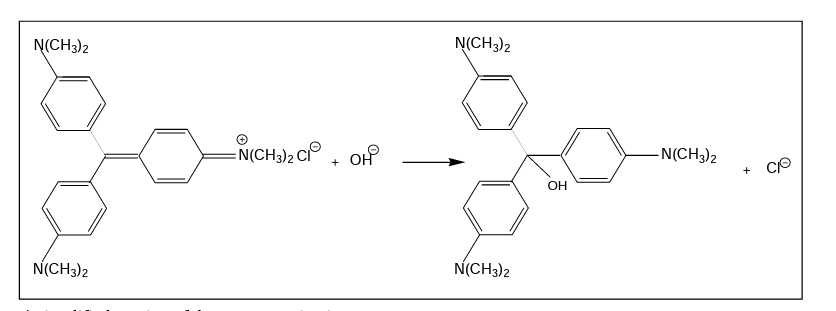
\includegraphics[width=0.9\textwidth]{reac.png}
\end{center}
\caption{Метиловый фиолетовый в средах с разным значением рН.}
\end{figure}
\subsection{Определение константы скорости из спектрофотометрических измерений}
\textbf{Закон светопоглощения Бугера-Ламберта-Бера}:
\begin{equation}
D = lg\frac{I}{I_{0}} = \varepsilon_{\lambda}Cl,
\end{equation}
где D -- оптическая плотность; $I_{0}$-- интенсивность падающего света; I -- интенсивность
света, прошедшего через образец; C -- концентрация вещества; l -- толщина
поглощающего слоя; $\varepsilon_{\lambda}$ -- коэффициент молярной экстинкции при длине волны $\lambda$.
Для реакции первого или псевдопервого порядка константа скорости:
\begin{equation}
k_{1} = \frac{1}{t} \cdot \ln \frac{C_{0}}{C(t)} = \frac{1}{t} \cdot \ln \frac{D_{0}}{D(t)},
\end{equation}
где $D_{0}$ -- начальная величина оптической плотности, $D(t)$ -- ее значение к моменту времени t.
\subsection{Влияние среды на скорость ионных реакций}

Реакции между заряженными частицами в растворах сопровождаются рядом специфических эффектов, обусловленных наличием электростатических взаимодействием ионов друг с другом и со средой, наиболее важными свойствами являются диэлектрическая проницаемость $\varepsilon$ и ионная сила J\\
В теории переходного состояния или активированного комплекса скорость
химической реакции:
\begin{equation}
W = (k_{\text{Б}}T/h)\cdot C^{\#}
\end{equation}
где $C^{\#}$ -- концентрация активированного комплекса. Множитель $k_{\text{Б}}T/h$ -- независящая от природы реагентов частота перехода комплексов через вершину активационного барьера.

Так как в данной теории постулируется существование равновесия между
исходными реагентами и активированным комплексом, концентрацию последнего
получаем, используя расчет констант
равновесия $K_{a}^{\#}$. Для бимолекулярной реакции с участием заряженных частиц A и B в растворе:
\begin{equation}
K_{a}^{\#} = (a^{\#}/a_{A}a_{B}) = (C^{\#}/C_{A}C_{B})\cdot (f^{\#}/f_{A}f_{B}),
\end{equation}
a и f -- активности и коэффициенты активности реагентов
и активированного комплекса $(a_{i} = f_{i}C_{i})$, его концентрация:
\begin{equation}
C^{\#} = K_{a}^{\#}(f_{A}f_{B}/f^{\#})C_{A}C_{B},
\end{equation}
Выражение для константы скорости реакции:
\begin{equation}
k = W/(C_{A}C_{B}) = (k_{\text{Б}}T/h)K_{a}^{\#}(f_{A}f_{B}/f^{\#}) = k_{0}(f_{A}f_{B}/f^{\#}),
\end{equation}
где в $k_{0}$ включены все независимые от свойств среды параметры.
Коэффициенты активности ионов в теории сильных электролитов
Дебая-Хюккеля, где для воды $(\varepsilon = 78,25)$ при Т = 298 К:
\begin{equation}
-\lg f_{i} \cong 0,51 Z_{i}^{2}J^{1/2}
\end{equation}
С учетом $Z^{\#} = Z_{A} + Z_{B}$:
\begin{equation}
\lg \frac{k}{k_{0}} \cong 1,02 Z_{A}Z_{B}J^{1/2}
\end{equation}
В случае одноименно
заряженных ионов $(Z_{A}Z_{B} > 0)$ константа скорости реакции растет с ионной силой, в случае разноименных $(Z_{A}Z_{B} < 0)$ -- уменьшается
\section{Ход работы и обработка данных}

\subsection{Снятие спектра поглощения красителя}

При помощи спектрофотометра получен спектр поглощения красителя (Рис 2.). Максимум поглощения находится на длине волны $\lambda$ = 591 нм. Дальнейшие измерения кинетики производятся на данной длине волны.

\begin{figure}[h!]
\begin{center}
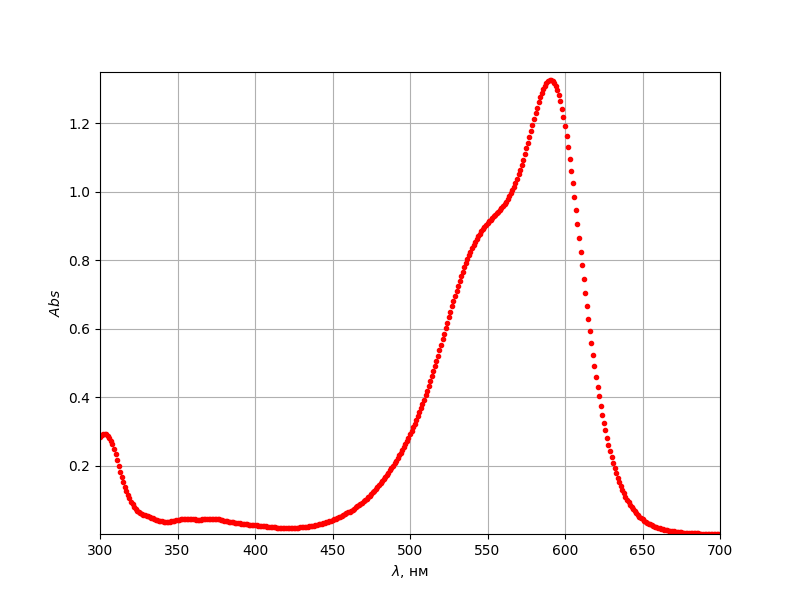
\includegraphics[width = 0.72\linewidth]{Figure_1.png}
\end{center}
\caption{Спектр поглощения метилового фиолетового.}
\end{figure}

\newpage

\subsection{Исследование зависимости скорости обесцвечивания красителя от концентрации щелочи.}
\begin{enumerate}
    \item На измеренной длине волны были сняты зависимости оптической плотности раствора от времени для растворов с разной концентрацией $\mathrm{NaOH}$. Ионная сила раствора при этом сохранялась постоянной путем добавления соответствующих количеств водного раствора хлорида натрия (Таблица 1). По полученным данным были построены графики зависимости $ln(D_0/D)$ от $t$. Сделаем предположения: во-первых, что концентрация $OH^{-}$ много больше чем коцентрация красителя и, следовательно,  мы можем считать ее  не меняющейся в течение прохождения реакции в каждом отдельном случае, и, во-вторых, что реакция имеет первый порядок по красителю. Тогда получаем, что в полулогарифмических координатах вид зависимости скорости реакции(прямо пропорциональной оптической плотности раствора) от времени - прямая линия, тангенс угла наклона которой соответствует эффективной константе скорости с точностью до знака (Рисунок 3). В Таблице 2 приведены полученные из аппроксимации по МНК прямыми в полулогарифмических координатах данных за первые $t = 200 c$ эффективные константы скорости для разных концентраций $NaOH$.

\begin{table}[h!]
\centering
\begin{tabular}{|
>{\columncolor[HTML]{FFFFFF}}r |
>{\columncolor[HTML]{FFFFFF}}r |
>{\columncolor[HTML]{FFFFFF}}r |
>{\columncolor[HTML]{FFFFFF}}r |
>{\columncolor[HTML]{FFFFFF}}l |}
\hline
\multicolumn{1}{|l|}{\cellcolor[HTML]{FFFFFF}{\color[HTML]{000000} $C_{0 NaOH}$,M}} & \multicolumn{1}{l|}{\cellcolor[HTML]{FFFFFF}{\color[HTML]{000000} $C_{0 NaCl}$,M}} & \multicolumn{1}{l|}{\cellcolor[HTML]{FFFFFF}{\color[HTML]{000000} $V_{NaOH}$,мкл}} & \multicolumn{1}{l|}{\cellcolor[HTML]{FFFFFF}{\color[HTML]{000000} $V_{NaCl}$,мкл}} & {\color[HTML]{000000} $V_{H2O}$,мл} \\ \hline
{\color[HTML]{000000} 0.001}                                                        & {\color[HTML]{000000} 0.099}                                                       & {\color[HTML]{000000} 10.0}                                                        & {\color[HTML]{000000} 990.0}                                                       & {\color[HTML]{000000} 2}            \\ \hline
{\color[HTML]{000000} 0.002}                                                        & {\color[HTML]{000000} 0.098}                                                       & {\color[HTML]{000000} 21.5}                                                        & {\color[HTML]{000000} 978.5}                                                       & {\color[HTML]{000000} 2}            \\ \hline
{\color[HTML]{000000} 0.005}                                                        & {\color[HTML]{000000} 0.095}                                                       & {\color[HTML]{000000} 46.4}                                                        & {\color[HTML]{000000} 953.6}                                                       & {\color[HTML]{000000} 2}            \\ \hline
{\color[HTML]{000000} 0.010}                                                        & {\color[HTML]{000000} 0.090}                                                       & {\color[HTML]{000000} 100.0}                                                       & {\color[HTML]{000000} 900.0}                                                       & {\color[HTML]{000000} 2}            \\ \hline
{\color[HTML]{000000} 0.022}                                                        & {\color[HTML]{000000} 0.078}                                                       & {\color[HTML]{000000} 215.4}                                                       & {\color[HTML]{000000} 784.6}                                                       & {\color[HTML]{000000} 2}            \\ \hline
{\color[HTML]{000000} 0.046}                                                        & {\color[HTML]{000000} 0.054}                                                       & {\color[HTML]{000000} 464.2}                                                       & {\color[HTML]{000000} 535.8}                                                       & {\color[HTML]{000000} 2}            \\ \hline
{\color[HTML]{000000} 0.100}                                                        & {\color[HTML]{000000} 0}                                                           & {\color[HTML]{000000} 1000.0}                                                      & {\color[HTML]{000000} 0}                                                           & {\color[HTML]{000000} 2}            \\ \hline
\end{tabular}
\caption{Расчет концентраций растворов для поддержания постоянной ионной силы $I = 0.1 M$.}
\label{tab:my-table}
\end{table}


\begin{figure}[h!]
\begin{center}
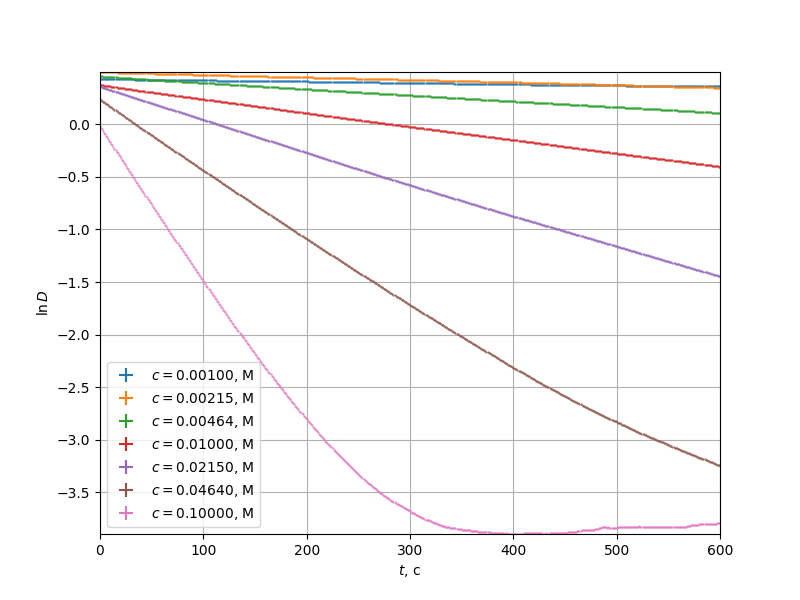
\includegraphics[width = 0.8\linewidth]{conc.png}
\end{center}
\caption{Кинетические кривые $ln(D_0/D)(t)$}
\end{figure}


\begin{table}[h!]
\centering
\begin{tabular}{|l|l|r|}
\hline
$\ln(C_{0NaOH})$ & $10^{6} \cdot k_{2} $, 1/c & \multicolumn{1}{l|}{$\ln ( k_{2}) $} \\ \hline
-6.908           & 115                        & -9.071                               \\ \hline
-6.14            & 257                        & -8.266                               \\ \hline
-5.373           & 606                        & -7.409                               \\ \hline
-4.605           & 1326                       & -6.626                               \\ \hline
-3.838           & 3144                       & -5.762                               \\ \hline
-3.07            & 6624                       & -5.017                               \\ \hline
-2.303           & 14070                      & -4.264                               \\ \hline
\end{tabular}
\caption{Эффективные константы скоростей реакций в зависимости от концентрации добавляемого $NaOH$.}
\label{tab:my-table}
\end{table}



\item Построим график зависимости эффективной константы скорости от концентрации $\mathrm{NaOH}$. Вследствие предположений, изложенных в первом пункте, получаем: $k_1 = k_2[OH^{-}]^n$, и в логарифмических координатах эта зависимость имеет вид прямой:
\[\ln k_{1}=\ln k_{2}+n \ln [\mathrm{OH}^-]\]
Построим эту зависимость (Рисунок 4) по полученным данным (Таблица 2), из нее определим по методу наименьших квадратов порядок реакции по $OH^{-}$: $n=1.05\approx1$ и $\ln k_{1} = -1.795$. Откуда $k_{1} =0.166127 \text{ M}^{-1.05}\text{c}^{-1}$.


\begin{figure}[h!]
\begin{center}
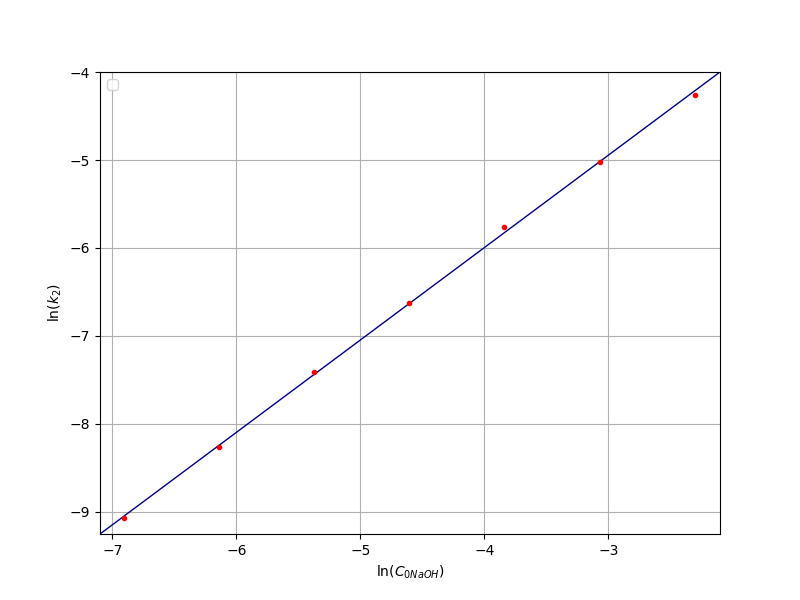
\includegraphics[width = 0.65\linewidth]{conc_1.png}
\end{center}
\caption{График зависимости логарифма константы скорости реакции $k_{2}$ от логарифма концентрации $\mathrm{NaOH}$}
\end{figure}

\end{enumerate}

\newpage

\subsection{Исследование зависимости кинетики реакции от ионной силы раствора $I$}

В этом опыте были проведены измерения скоростей реакций при
различной ионной силе раствора, которая варьировалась разным составом смеси (Таблица 3). По полученным данным (Таблица 4, Рисунок 5) были построены графики (Рисунок 6, 7) зависимости в первом и втором приближениях теории Дебая-Хюккеля. По линеаризованным зависимостям по МНК были получены значения коэффициентов углов наклона: для первого приближения $k^{1} = -1.175$, для второго $k^{2} = -2.567$. Согласно расчетам констант скоростей реакций по моделе Дебая для медленных (лимитирует стадия химической реакции) реакций в случае концентрированных растворов электролитов имеем: $\ln(\frac{k}{k_{0}}) = 2z_{A}z_{B} \cdot \frac{A \sqrt{I}}{1+B\sqrt{I}}$, где коэффициенты $A$ и $B$ расчитываются согласно теории сильных электролитов Дебая-Хюккеля. В нашем случае (растворитель - вода, $T = 293 К$, центральный ион большой и несимметричный): $A = 1.17 M^{-1/2}$, $B \approx 1 M^{-1/2}$. В первом приближении получаем: $k^{1} = 2z_{A}z_{B} \cdot A $, тогда по полученным значениям имеем $z_{A}z_{B} = -0.50 $. Во втором приближении: $k^{2} = 2z_{A}z_{B} \cdot A $, тогда $z_{A}z_{B} = -1.10$. В силу несимметричности ионов в растворе и больших значений ионной силы, более правильно использование второго приближения теории Дебая-Хюккеля, подтверждение чему мы видим по полученным данным.
 
\begin{table}[h!]
\centering
\begin{tabular}{|r|r|r|r|}
\hline
\multicolumn{1}{|l|}{$I$, М} & \multicolumn{1}{l|}{$C_{0NaCl}$, М} & \multicolumn{1}{l|}{$V_{0NaCl}$, мкл} & \multicolumn{1}{l|}{$C_{0H2O}$, мкл} \\ \hline
0.01                         & 0                                   & 0                                     & 1900                                 \\ \hline
0.0625                       & 0.0525                              & 65.6                                  & 1834.4                               \\ \hline
0.16                         & 0.15                                & 187.5                                 & 1712.5                               \\ \hline
0.3025                       & 0.2925                              & 365.6                                 & 1534.4                               \\ \hline
0.49                         & 0.48                                & 600                                   & 1300                                 \\ \hline
0.7225                       & 0.7125                              & 890.6                                 & 1009.4                               \\ \hline
1                            & 0.99                                & 1237.5                                & 662.5                                \\ \hline
\end{tabular}
\caption{Расчет концентраций растворов для изменения ионной силы растворов при поддержания постоянной концентрации $NaOH$: $C_{0NaOH} = 0.01 М$.}
\label{tab:my-table}
\end{table}



\begin{table}[h!]
\centering
\begin{tabular}{|r|r|r|r|r|}
\hline
\multicolumn{1}{|l|}{$I$, М} & \multicolumn{1}{l|}{$\sqrt{I}$, М} & \multicolumn{1}{l|}{$ \frac{\sqrt{I}}{1+\sqrt{I}}$} & \multicolumn{1}{l|}{$10^{-4} \cdot k$} & \multicolumn{1}{l|}{$\ln (k) $} \\ \hline
0.0100                       & 0.10                               & 0.091                                               & 19.08                                   & -6.262                          \\ \hline
0.0625                       & 0.25                               & 0.200                                               & 16.19                                   & -6.426                          \\ \hline
0.1600                       & 0.40                               & 0.286                                               & 12.39                                   & -6.693                          \\ \hline
0.3025                       & 0.55                               & 0.355                                               & 10.91                                   & -6.821                          \\ \hline
0.4900                       & 0.70                               & 0.412                                               & 9.838                                   & -6.924                          \\ \hline
0.7225                       & 0.85                               & 0.459                                               & 7.871                                   & -7.147                          \\ \hline
1.0000                       & 1.00                               & 0.500                                               & 6.429                                   & -7.35                           \\ \hline
\end{tabular}
\caption{Эффективные константы скоростей в зависимости от ионной силы раствора и расчеты для проверки теории Дебая-Хюккеля в 1 и 2 приближениях.}
\label{tab:my-table}
\end{table}

\begin{figure}[H!]
\begin{center}
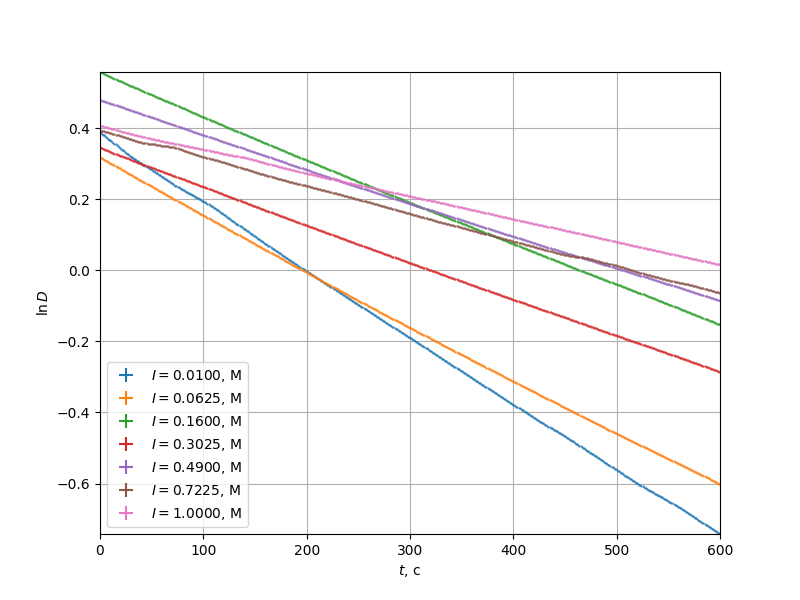
\includegraphics[width = 0.75\linewidth]{ion_1.png}
\end{center}
\caption{Кинетические кривые $ln(D_0/D)(t)$ для различных значений ионной силы}
\end{figure}

\begin{figure}[H!]
\begin{center}
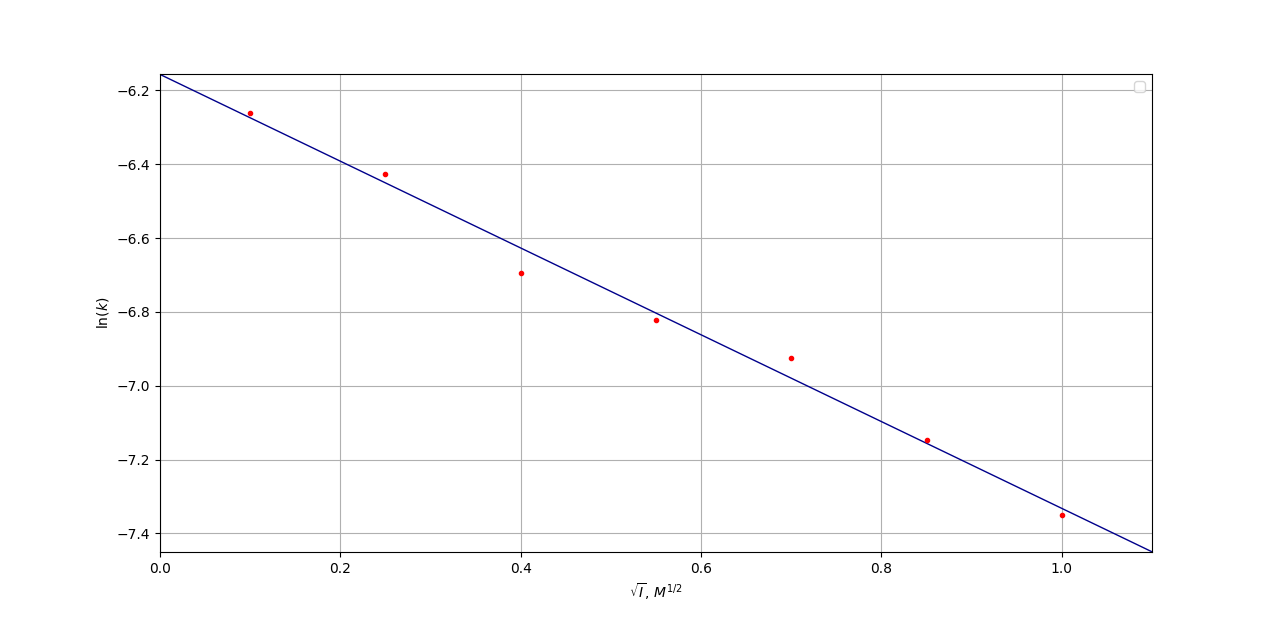
\includegraphics[width = 0.9\linewidth]{ion_2.png}
\end{center}
\caption{График зависимости логарифма констант скоростей реакций $\ln k$ от корня из ионной силы $\sqrt {I}$.Первое приближение теории Дебая-Хюккеля. }
\end{figure}

\begin{figure}[h!]
\begin{center}
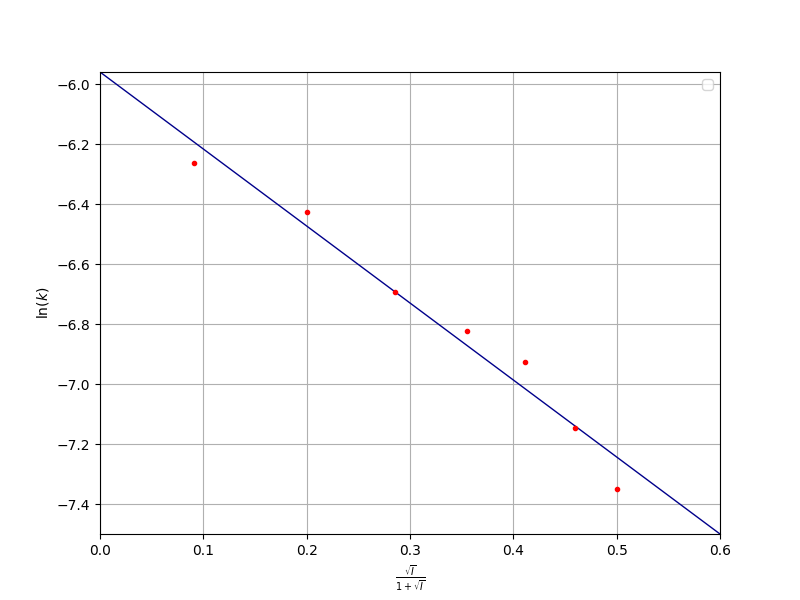
\includegraphics[width = 0.75\linewidth]{ion_3.png}
\end{center}
\caption{График зависимости логарифма констант скоростей реакций $\ln k$ от $ \frac{\sqrt{I}}{1+\sqrt{I}}$.Второе приближение теории Дебая-Хюккеля.}
\end{figure}


\newpage

\section{Обсуждение результатов и выводы}
\begin{itemize}
    \item Снят спектр поглощения метилового фиолетового, максимальное поглощение происходит при длине волны $\lambda = 591$ \text{нм}, соответствующей оранжево-желтому цвету, вследствие чего наблюдаемый цвет красителя - сине-голубой. 
    \item В предположении хода реакции в первоим порядке по красителю (что мы заключили из поведения графика зависимости логарифма оптической плотности раствора от времени, который представлял собой прямую в начальные моменты времени) и избыточной концентрации ионов $OH^{-}$, был получен порядок реакции по  $OH^{-}$: $n = 1.05$ и определена истинная константа скорости реакции: $k_{1} =0.166127 \text{ M}^{-1.05}\text{c}^{-1}$. 
    \item Во второй части работы было исследовалось влияние ионной силы на кинетику обесцвечивания метилового фиолетового. Построение зависимостей констант скоростей реакций от $\sqrt{I}$ и $\frac{\sqrt{I}}{1+\sqrt{I}}$ показало, что первое приближение теории Дебая-Хюккеля в нашем случае работает хуже, чем второе. Экспериментально подтвердили разноименность ионов, присутствующих в растворе и вступащих в реакцию (краситель и $OH^{-}$) (полученные коэффициенты углов наклона прямых $k^{1}, k^{2}$ меньше нуля). Также видно, что при увеличении ионной силы раствора скорость реакции уменьшается - следствие разноименности взаимодействующих частиц и зависимости радиуса ионной атмосферы от ионной силы.
    
\end{itemize}






\newpage

\addcontentsline{toc}{section}{Список используемой литературы}
\begin{thebibliography}{}
     \bibitem{2}  Департамент химии МФТИ -  "Кинетика обесцвечивания красителей"
    \bibitem{1} Общедоступная многоязычная универсальная интернет-энциклопедия Википедия - 
$https://en.wikipedia.org/wiki/Methyl_violet$
\end{thebibliography}




\end{document}
